\section{External descriptive evidence}

\subsection{Purpose and construction}

The external analysis asks whether score--acreage disagreement is visible
beyond the Kansas calibration. It does not treat observed state acreage as a
solution to Eq.~\ref{eq:canonical}. USDA NASS annual state reports yield
\StateYears{} complete state-years across \States{} states from 2016 through
2024 for corn, soybean and winter wheat. National harvest prices and operating
and total costs come from USDA ERS, and BLS CPI-U supplies the real-dollar
conversion. Suppressed or missing acreage and yield are not imputed.

Four ranking definitions are computed before comparison with planted-acreage
share. Relative yield is state yield divided by same-year national yield.
Standardized revenue multiplies state yield by national price. Operating
margin subtracts national operating cost; total-cost margin subtracts total
cost. The latter three are transparent accounting measures rather than local
or private expected profits. For each state-year we calculate pairwise
inversion intensity and whether the top-ranked crop differs from the acreage
leader. State-cluster bootstrap intervals preserve within-state serial
dependence.

\subsection{Descriptive prevalence and definition sensitivity}

Top-rank disagreement is \RelativeYieldRate{} for relative yield,
\RevenueRate{} for standardized revenue, \OperatingMarginRate{} for operating
margin and \TotalCostRate{} for total-cost margin. The corresponding
state-cluster intervals are all well above zero. The ordering across
definitions is itself a result: a claim about ranking reversal inherits the
scientific meaning of the score being ranked. Relative-yield disagreement
cannot be interpreted as profit inefficiency, while a margin-based
disagreement remains incomplete because local basis, heterogeneous costs,
contracts, beliefs and risk limits are unobserved.

The leakage-free temporal check uses prior relative-yield potential to predict
the following change in acreage share with crop, state and decision-year fixed
effects. It includes 651 crop-transition rows. The estimated effect is
\LaggedEffect{} share units with interval
\([\LaggedLow,\LaggedHigh]\), which includes zero. Thus the panel does not
show that a crop's earlier score leadership leads to a larger next-year share
change. This null is consistent with many mechanisms, including persistent
rotations, adjustment cost and a score that does not measure private profit;
it is not evidence that agronomic information has no value.

\begin{figure}[t]
\centering
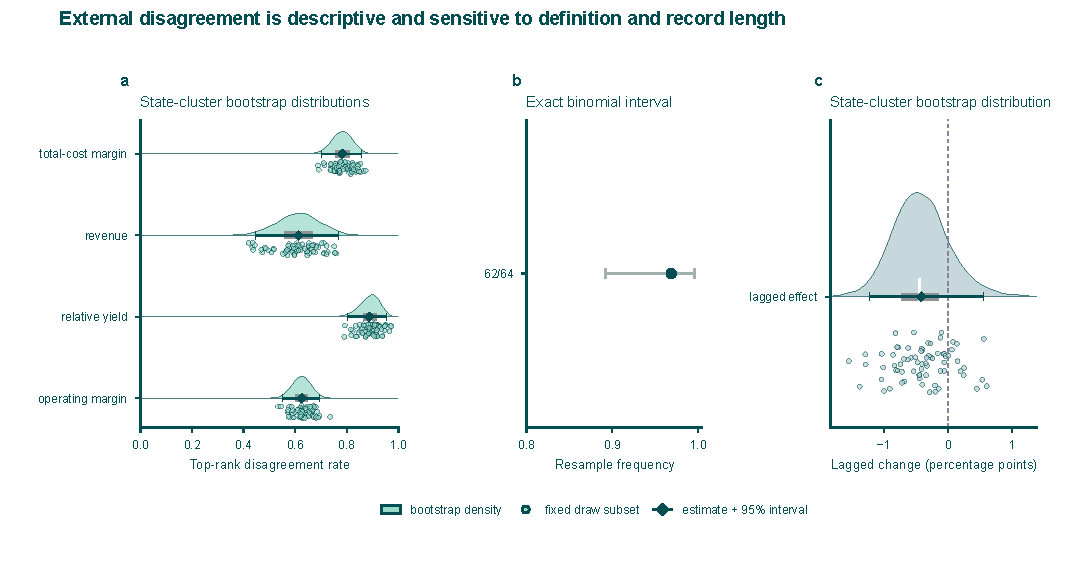
\includegraphics[width=\textwidth]{figures/issue34/Figure6.pdf}
\caption{\textbf{External patterns support prevalence, not causal mechanism
attribution.} \textbf{a}, Top-rank disagreement rates and state-cluster 95\%
intervals in \StateYears{} state-years. \textbf{b}, Historical resampling of
the calibrated full model shows allocation uncertainty and reversal
probability \BootstrapProbability. \textbf{c}, the eight-year dependence
estimate has a wide interval; copula parameters are therefore stress paths,
not farm-level tail estimates.}
\label{fig:external}
\end{figure}

\subsection{Evidence boundary}

The external layer validates three limited propositions. Score--acreage
disagreement exists at a meaningful scale; it varies across definitions; and
aggregate data do not show a leakage-free lagged response to the genuine
relative-yield score. It does not identify the full model's CVaR mechanism,
estimate private risk aversion, reveal the active constraint set, or establish
welfare. Those claims require farm-level expectations, resource capacities,
contract terms and decision timing. Treating the state panel as descriptive
is not a weakness to hide; it prevents aggregate acreage from being used to
``confirm'' a mechanism that it cannot identify.
